\documentclass[11pt,a4paper]{article}
\usepackage[margin=2.5cm]{geometry}
\usepackage{amsmath,amssymb}
\usepackage{booktabs}
\usepackage{array}
\usepackage{xcolor}
\usepackage{tcolorbox}
\tcbuselibrary{skins,breakable}
\usepackage{hyperref}
\usepackage[numbers,sort&compress]{natbib}
\bibliographystyle{unsrtnat}
\usepackage{microtype}
\usepackage{enumitem}
\usepackage{tabularx,ragged2e}
\usepackage{tikz}
\usetikzlibrary{arrows.meta,positioning,calc,decorations.pathreplacing}
\newcolumntype{P}[1]{>{\RaggedRight\arraybackslash}p{#1}}

\hypersetup{colorlinks=true,linkcolor=blue!60!black,urlcolor=blue!60!black,
            citecolor=blue!60!black}

\definecolor{boxblue}{RGB}{220,235,255}
\definecolor{boxorange}{RGB}{255,240,210}
\definecolor{boxgreen}{RGB}{220,245,220}
\definecolor{boxred}{RGB}{255,228,225}
\definecolor{boxgray}{RGB}{242,242,242}

\newcommand{\term}[1]{\textbf{#1}}
\newcommand{\lean}[1]{\begingroup\def\_{\textunderscore\allowbreak}\texttt{#1}\endgroup}
\newcommand{\GN}{G_{\!N}}
\newcommand{\MPl}{M_{\rm Pl}}
\newcommand{\mtau}{m_\tau}
\newcommand{\PHIMDL}{\Phi_{\mathrm{MDL}}}
\newcommand{\ZS}{\mathbb{Z}_7}

\title{\textbf{Gravity from Description-Length Minimization}\\[6pt]
\large The MDL-Lovelock Principle and the GTE Derivation of General Relativity\\[4pt]\normalsize\textit{UGP Physics Tutorial Series}
\\[2pt]\small\href{https://doi.org/\TutorialDOI}{doi.org/\TutorialDOI}}
\author{Nova Spivack\\[4pt]
\normalsize
\href{https://novaspivack.com/research}{novaspivack.com/research}\\[2pt]
\small Full corpus (P00--P51):
\href{https://doi.org/10.5281/zenodo.20171558}{doi.org/10.5281/zenodo.20171558}
}
\newcommand{\TutorialDOI}{10.5281/zenodo.20657870}
\date{2026}

\begin{document}
\setcounter{tocdepth}{2}
\maketitle
\tableofcontents
\newpage

\begin{tcolorbox}[colback=blue!6,colframe=blue!40!black,
  title=\textbf{UGP Physics Tutorial Series}]
\textbf{Prerequisites (read first):} \href{https://doi.org/10.5281/zenodo.20657885}{\emph{The $\Phi_{\rm MDL}$ Field}} $\cdot$ \href{https://doi.org/10.5281/zenodo.20657906}{\emph{The Three-Tape CMCA}}\\[4pt]
\textbf{Next tutorials:} \href{https://doi.org/10.5281/zenodo.20657864}{\emph{The Cosmological Constant}}\\[4pt]
\textbf{See also:} \href{https://doi.org/10.5281/zenodo.20657861}{\emph{The Born Rule as a Theorem}}
\end{tcolorbox}

\begin{tcolorbox}[colback=boxgreen,colframe=green!50!black,
  title=\textbf{Claim-Strength Taxonomy}]
Throughout this tutorial, results are labeled with a confidence grade:
\begin{itemize}[itemsep=2pt]
  \item \textbf{$\mathbf{A}_{\rm Lean}$ (CatAL)} --- Machine-certified in Lean~4 with zero \texttt{sorry} and zero custom axioms.  Independently verifiable by anyone with Lean installed.
  \item \textbf{A/D (CatAD)} --- Analytically derived with full derivation, computationally confirmed.  Not yet machine-certified.
  \item \textbf{A (CatA)} --- Analytically derived; derivation complete but not independently machine-certified.
  \item \textbf{A/D (conditional)} --- Derived under a named, stated premise; the premise is itself an open problem or a CatB assumption.
  \item \textbf{B (CatB)} --- A stated working hypothesis or structural premise; not yet derived.
\end{itemize}
\end{tcolorbox}


%─────────────────────────────────────────────────────────────────────────────
\section{The Problem: Why Gravity is Different}
%─────────────────────────────────────────────────────────────────────────────

\begin{tcolorbox}[colback=boxblue,colframe=blue!40!black,title=The puzzle in one sentence]
Every other force in nature is described by a quantum field theory; gravity alone
is still described by a classical (non-quantum) theory, and the two are mathematically
incompatible at the highest energies.
\end{tcolorbox}

\subsection{The four forces and how we describe them}

Physics currently knows of four fundamental forces: gravity, electromagnetism, and the
strong and weak nuclear forces.  For the last three, the most successful description
we have is \term{quantum field theory} (QFT): fields fill all of space, particles are
excitations of those fields, and the forces arise from the exchange of force-carrying
particles (photons for electromagnetism, gluons for the strong force, W and Z bosons
for the weak force).  This framework is extraordinarily accurate---predictions match
measurements to twelve decimal places in some cases.

Gravity refuses to fit this pattern.  Our best description of gravity is
\term{general relativity} (GR), a classical theory that says
\emph{massive objects curve spacetime itself, and other objects follow the
curves}.  GR is also extraordinarily accurate: it predicted the bending of starlight
around the Sun, the precession of Mercury's orbit, and gravitational waves from
merging black holes, all confirmed to high precision.

The problem is that GR and QFT are \emph{incompatible} at very high energies (near
the \term{Planck scale}, $\sim10^{19}$ GeV).  When you try to combine them---to
describe what happens when quantum particles interact gravitationally in extreme
conditions, such as at the centre of a black hole or at the moment of the Big Bang---the
equations produce infinities that cannot be removed.  Every other force's infinities
were cured by a procedure called \emph{renormalization}; gravity's cannot.

\subsection{What ``quantum gravity'' is trying to achieve}

A \term{theory of quantum gravity} aims to describe gravity and quantum mechanics
within a single consistent framework.  The two leading contenders---string theory and
loop quantum gravity---take opposite strategies.

\medskip
\noindent\textit{String theory} starts from the top: replace point particles with tiny
vibrating strings, and one of the string vibration modes automatically behaves like a
graviton (the force carrier of gravity).  It works, but only in ten or eleven
dimensions; six or seven extra dimensions must be hidden away, and the theory has a
vast ``landscape'' of possible universes with no principle to select ours.

\medskip
\noindent\textit{Loop quantum gravity} starts from the bottom: quantize spacetime
itself, so that space is made of discrete chunks of area (``spin foam'').  It
avoids the extra dimensions but has trouble recovering standard QFT at low energies
and has not yet derived the Standard Model.

Both approaches quantize GR from \emph{outside}: they take Einstein's equations as
given and try to make them compatible with quantum mechanics.

\medskip
\begin{tcolorbox}[colback=boxgreen,colframe=green!50!black,title=The GTE approach]
The GTE framework~\cite{SpivackGTECompleteFramework} takes a different route: instead of quantizing GR from outside,
it \emph{derives} GR from below---from a deeper discrete structure---without
ever postulating Einstein's equations.
The equations emerge as a theorem about information minimization.
\end{tcolorbox}

%─────────────────────────────────────────────────────────────────────────────
\section{How General Relativity Works: The Key Ideas}
%─────────────────────────────────────────────────────────────────────────────

\begin{tcolorbox}[colback=boxblue,colframe=blue!40!black,title=The two-sentence summary of GR]
Mass (and energy) curves spacetime.
Objects move along the straightest possible paths through that curved spacetime.
\end{tcolorbox}

\subsection{Spacetime: putting space and time together}

Before Einstein, physicists thought of space and time as separate and absolute.
Space was a fixed three-dimensional arena; time ticked uniformly for everyone.
Einstein's \term{special relativity} (1905) showed that this is wrong: moving clocks
run slow, moving rulers shrink, and two observers moving at different speeds disagree
about whether two events happen at the same time.

What stays the same for all observers is not space alone, and not time alone, but
a combined quantity called the \term{spacetime interval}:
\[
  s^2 = -c^2\,(\Delta t)^2 + (\Delta x)^2 + (\Delta y)^2 + (\Delta z)^2.
\]
This four-dimensional arena---three spatial dimensions plus one time dimension---is
\term{spacetime}, and it has signature $(+,+,+,-)$.  The minus sign in front of
$(\Delta t)^2$ is not a typo; it is what makes the time direction fundamentally
different from the three space directions.

\subsection{Curved spacetime and the rubber-sheet analogy}

\term{General relativity} (1915) extended this to include gravity.  The central
insight is that mass---or more precisely, \emph{energy and momentum}---warps the
geometry of spacetime.

The classic illustration is the \term{rubber-sheet analogy}: imagine spacetime as
a stretched rubber sheet.  Place a heavy bowling ball (a star or planet) on the
sheet; it creates a depression.  A smaller marble (a planet or comet) rolling nearby
does not follow a straight line; it curves toward the bowling ball, following the
contour of the sheet.  That curvature \emph{is} what we call gravitational attraction.

\medskip
\begin{center}
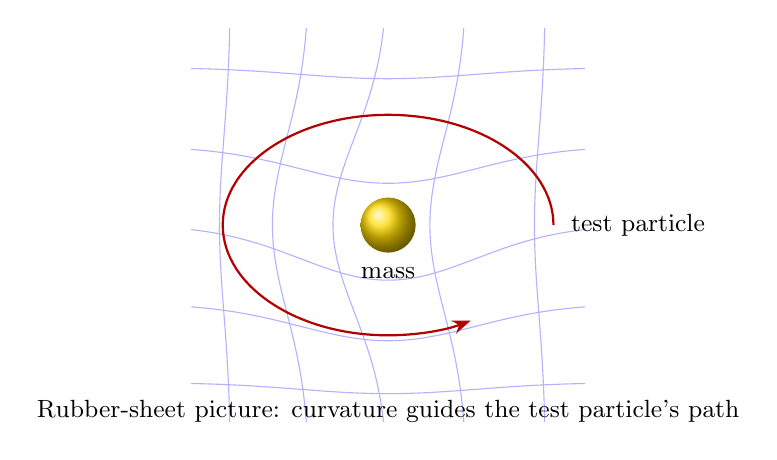
\begin{tikzpicture}[scale=1.0]
  % Draw curved grid representing spacetime curvature
  \foreach \i in {-2,-1,0,1,2}{
    \draw[blue!30,thin] plot[smooth,samples=30,domain=-2.5:2.5]
      (\x,{\i-0.7*exp(-0.4*(\x*\x+\i*\i))});
  }
  \foreach \i in {-2,-1,0,1,2}{
    \draw[blue!30,thin] plot[smooth,samples=30,domain=-2.5:2.5]
      ({\i-0.7*exp(-0.4*(\i*\i+\x*\x))},\x);
  }
  % Central mass
  \shade[ball color=yellow!70!orange] (0,0) circle (0.35);
  \node[below=2pt] at (0,-0.35) {\small mass};
  % Orbit path (ellipse approximation)
  \draw[red!70!black,thick,->,>=Stealth]
    (2.1,0) arc[start angle=0,end angle=300,x radius=2.1,y radius=1.4];
  \node[right] at (2.2,0) {\small test particle};
  % Label
  \node[below] at (0,-2.1)
    {\small Rubber-sheet picture: curvature guides the test particle's path};
\end{tikzpicture}
\end{center}

\medskip
The rubber-sheet picture has a limitation: the sheet is two-dimensional and lives
in three-dimensional space, while real spacetime is four-dimensional with no
``outside'' to curve into.  The curvature is \emph{intrinsic}---detectable by
measurements made entirely within spacetime, without needing to embed it in anything
larger.

\subsection{Geodesics: straightest paths in curved spacetime}

In flat (uncurved) spacetime, a free particle moves in a straight line at constant
speed---this is just Newton's first law.
In curved spacetime, the analogue of a straight line is called a \term{geodesic}:
the path of shortest distance (or, for timelike paths, longest proper time) between
two events.

Think of the surface of the Earth.  The shortest path between two cities is a
great circle arc, even though it looks curved on a flat map.  A great circle is the
geodesic on a sphere.  In the same way, a planet orbiting the Sun follows a geodesic
of the curved spacetime around the Sun---it is not ``pulled'' by a force but is
instead taking the straightest available path through curved geometry.

\subsection{Einstein's equation}

The mathematical heart of GR is \term{Einstein's field equation}:
\begin{equation}
  G_{\mu\nu} + \Lambda\, g_{\mu\nu} = 8\pi\GN\, T_{\mu\nu}.
  \label{eq:Einstein}
\end{equation}

\medskip
\begin{center}
\renewcommand{\arraystretch}{1.4}
\begin{tabular}{cll}
\toprule
Symbol & Name & What it means \\
\midrule
$G_{\mu\nu}$ & Einstein tensor & curvature of spacetime \\
$\Lambda$ & cosmological constant & ``dark energy'' / vacuum energy \\
$g_{\mu\nu}$ & metric tensor & the shape of spacetime itself \\
$\GN$ & Newton's constant & the strength of gravity \\
$T_{\mu\nu}$ & stress-energy tensor & energy, momentum, and pressure of matter \\
\midrule
\multicolumn{3}{c}{\textit{Left side = spacetime geometry; \quad Right side = matter content}} \\
\bottomrule
\end{tabular}
\end{center}
\medskip

In plain English: \emph{curvature (left) is sourced by energy and momentum (right)}.
The equation is usually \emph{postulated}---Einstein wrote it down guided by physical
intuition and mathematical requirements.  In GTE, it is a \emph{theorem}.

%─────────────────────────────────────────────────────────────────────────────
\section{The GTE Framework: Spacetime from Scratch}
%─────────────────────────────────────────────────────────────────────────────

\begin{tcolorbox}[colback=boxblue,colframe=blue!40!black,title=Starting point]
The GTE framework begins with a single cellular automaton rule on a one-dimensional
tape: $p(L,C,R) = C + R - CR - LCR$ over seven-element clock arithmetic.
From this single polynomial, with zero free parameters, spacetime emerges.
\end{tcolorbox}

\subsection{What is a cellular automaton?}

A \term{cellular automaton} (CA) is a row of cells, each holding a value.
At every tick of a clock, every cell simultaneously updates its value using a fixed
rule that looks only at its two nearest neighbours and itself.
Stephen Wolfram's Rule~110 (with two possible states, 0 or 1) is the simplest
computationally universal example.

The GTE polynomial uses seven states per cell ($\{0,1,2,3,4,5,6\}$, arithmetic
wrapping around modulo 7), and the update rule is:
\[
  p(L,C,R) = C + R - CR - LCR \pmod{7}.
\]
This 19-bit formula is the unique description of the observable particle physics
spectrum selected by the Minimum Description Length (MDL) principle.
Restricted to binary inputs ($\{0,1\}$), it reproduces Rule~110 exactly---inheriting
Turing universality.

\subsection{Levels: algebraic certificates and physical fields}

Two conceptual levels are essential throughout this tutorial.

\begin{itemize}[leftmargin=1.5em]
\item \textbf{Level~1 (algebraic certificate)}: the one-dimensional CA tape and its
  discrete arithmetic---Rule~110 orbits, $\mathbb{Z}_7$ winding numbers, orbit counts.
  This level produces exact theorems, many machine-certified in Lean~4.
\item \textbf{Level~2 (continuum physical substrate)}: $\PHIMDL$, a
  $\mathbb{Z}_7$-symmetric Klein-Gordon field in continuous spacetime.  Particles
  are topological solitons (kinks) in this field.  The physical world lives here.
\end{itemize}

A pair of theorems (the \emph{Algebraic Lifting and Descent Theorems}) guarantees that
every algebraic fact proved at Level~1 has a corresponding physical statement at
Level~2---so the CA certificates are not mere analogies but genuine mathematical
proofs about the physical field.

\subsection{The elevator analogy for why we need spacetime}

The CA tape is intrinsically one-dimensional: cells strung out on a line, ticking
forward in time.  That is $1{+}1$-dimensional---one space dimension, one time
dimension.  Real physics requires $3{+}1$ dimensions.

Think of an elevator shaft.  A single shaft gives one direction of travel.
Two shafts give two independent directions.
\emph{Three} shafts, all connected to the same clock and synchronized, give three
independent spatial directions.
In GTE, the CA runs on \emph{three tapes simultaneously}, with a shared outer clock.
This is the Chiral Minkowski Cellular Automaton (CMCA), and it produces exactly
$3{+}1$-dimensional spacetime.

Why three shafts and not two or four?  That is the content of the next section.

%─────────────────────────────────────────────────────────────────────────────
\section{Why 3+1 Dimensions? The Discrete Parity Pattern Argument}
%─────────────────────────────────────────────────────────────────────────────

\begin{tcolorbox}[colback=boxorange,colframe=orange!60!black,title=Key theorem]
Three spatial dimensions emerge because the polynomial has exactly three
generation types in its diagonal $p(w,w,w) = 2w - w^2 - w^3$, and each
generation type requires one independent spatial direction.
This is machine-certified in Lean~4 with zero sorry.
\end{tcolorbox}

\subsection{The diagonal of the polynomial and the generation count}

The polynomial $p(w,w,w)$ evaluated with all three inputs equal is:
\[
  p(w,w,w) = 2w - w^2 - w^3.
\]
This cubic encodes the three generations of matter (electron/muon/tau families in
the Standard Model).  A \term{Garden of Eden} (GoE) analysis---identifying
configurations with no predecessor under the update rule---shows that there are
exactly three GoE orbit types.  This forces:
\[
  N_{\rm gen} = 3
\]
as a theorem (\lean{three\_generations\_physical}, \texttt{ugp-lean}, machine-certified).

\subsection{From three generations to three spatial dimensions}

Each generation orbit type requires an independent spatial direction to encode its
causal history.  The argument is an MDL (Minimum Description Length) minimality
argument:

\begin{itemize}[leftmargin=1.5em,nosep]
\item \textit{Too few spatial dimensions:} a theory with only two spatial dimensions
  cannot accommodate all three generation orbit steps; some algebraic content is lost.
\item \textit{Too many spatial dimensions:} extra dimensions carry no generation
  content and therefore cost description-length bits without adding physical structure.
  MDL minimality excludes them.
\end{itemize}

The result is the theorem $N_{\rm gen} = 3 \Rightarrow D_{\rm spatial} = 3$
(\lean{three\_dim\_fmdl\_structure\_forced}, \texttt{ugp-lean}, machine-certified; P36).

\subsection{The Dimensional Protocol Principle: why a shared clock is essential}

Three CA tapes without synchronization are three independent one-dimensional
systems---they generate no spatial geometry between them.
A \term{shared outer clock} connecting the three tapes is both necessary and sufficient
to promote three $1{+}1$-dimensional systems to one $3{+}1$-dimensional system.

\begin{tcolorbox}[colback=boxgreen,colframe=green!50!black,
  title={Theorem: Dimensional Protocol Principle}]
A shared outer clock $\tau_c^{\rm out}$ is both necessary and sufficient for
three $1{+}1$-dimensional CMCAs to produce one $3{+}1$-dimensional Minkowski
dynamical system.\\[4pt]
Lean certifications (zero sorry):\\
\lean{dimensional\_protocol\_principle\_master} \quad (P45)\\
\lean{cmca\_tensor\_product\_gives\_31d\_minkowski} \quad (P45)
\end{tcolorbox}

The argument is intuitive: each tape contributes a pair of null directions
(right-moving and left-moving signals), corresponding to one spatial axis.
The shared clock provides the time coordinate.
Together, three tapes and one clock span $(x, y, z, t)$---exactly $3{+}1$D
with Minkowski signature $(+,+,+,-)$.

\medskip
\begin{center}
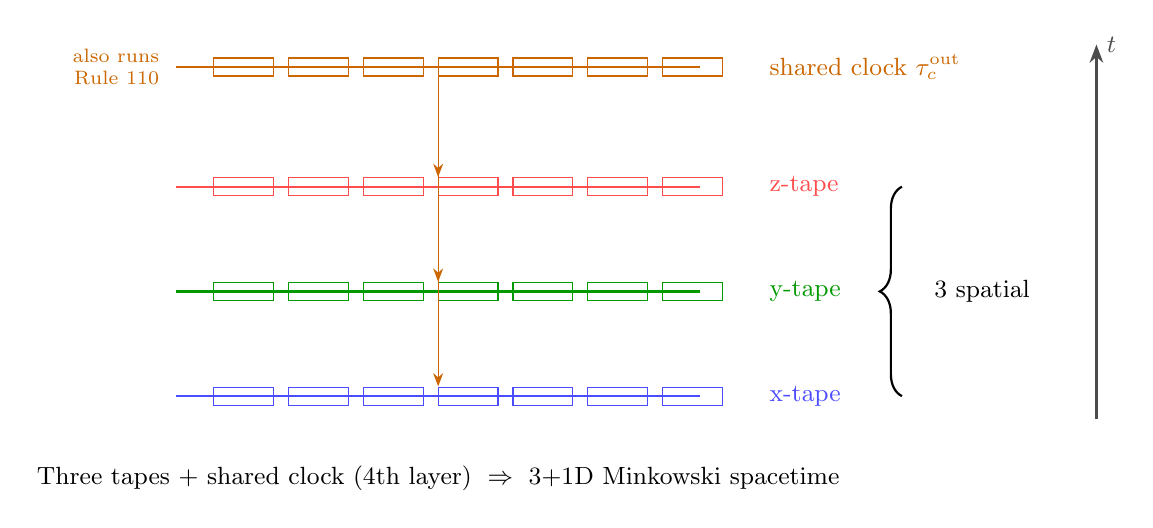
\begin{tikzpicture}[scale=0.95,>=Stealth]
  % Shared clock — 4th tape above the three spatial tapes
  \draw[orange!80!black,thick] (-3.5,4.4) -- (3.5,4.4);
  \foreach \i in {-3,-2,-1,0,1,2,3}{
    \draw[orange!80!black] (\i,4.4-0.12) rectangle (\i+0.8,4.4+0.12);
  }
  \node[right,orange!80!black] at (4.3,4.4) {\small shared clock $\tau_c^{\rm out}$};
  \node[left,orange!80!black,font=\scriptsize,align=right] at (-3.6,4.4)
    {also runs\\Rule~110};
  % Three spatial tapes
  \foreach \j/\col/\lbl in {0/blue!70/x-tape, 1.4/green!60!black/y-tape, 2.8/red!70/z-tape}{
    \draw[\col,thick] (-3.5,\j) -- (3.5,\j);
    \foreach \i in {-3,-2,-1,0,1,2,3}{
      \draw[\col] (\i,\j-0.12) rectangle (\i+0.8,\j+0.12);
    }
    \node[right,\col] at (4.3,\j) {\small\lbl};
  }
  % Synchronization arrows from clock to each tape
  \foreach \j in {0,1.4,2.8}{
    \draw[orange!80!black,thin,->] (0,4.28) -- (0,\j+0.13);
  }
  % Brace indicating 3 spatial tapes (moved right, clear of labels)
  \draw[decorate,decoration={brace,amplitude=8pt},thick]
    (6.2,0) -- (6.2,2.8) node[midway,right=8pt]{\small $3$ spatial};
  % Time arrow (further right, clear of brace label)
  \draw[thick,->,gray!60!black] (8.8,-0.3) -- (8.8,4.7)
    node[right]{\small $t$};
  \node[below] at (0,-0.8) {\small Three tapes + shared clock (4th layer) $\;\Rightarrow\;$ $3{+}1$D Minkowski spacetime};
\end{tikzpicture}
\end{center}

\subsection{Why not four dimensions?}

A fourth tape would introduce an extra spatial direction with no corresponding
generation orbit type.  The degree-3 diagonal $p(w,w,w)$ provides three orbit
steps---one per generation---and no fourth.  Adding a fourth tape therefore increases
the description length without adding physical structure.  MDL minimality excludes it.

The three-tape CMCA is the unique MDL-minimal sufficient construction for
$3{+}1$D spacetime.

\subsection{A triple identity: particles, computation, and spacetime}

A remarkable consequence is the \textit{PCT Trinity}: every PSC-admissible kink
simultaneously (a)~carries Standard Model quantum numbers, (b)~implements Boolean
computation, and (c)~sources spacetime curvature.  These are not three separate
roles; they are three facets of the same arithmetic structure.  This is why
$N_{\rm gen} = N_c = N_{\rm tapes} = 3$: all three counts refer to the
same degree-of-freedom structure of the polynomial.\\
(\lean{particles\_computation\_spacetime\_trinity}, \texttt{ugp-lean}, machine-certified; P45)

%─────────────────────────────────────────────────────────────────────────────
\section{Special Relativity from the CMCA: A Built-in Speed Limit}
%─────────────────────────────────────────────────────────────────────────────

\begin{tcolorbox}[colback=boxblue,colframe=blue!40!black,title=The key insight]
A CA has a built-in speed limit: information cannot propagate faster than one cell
per tick.  In the CMCA, this maximum speed is $c$.  Special relativity is not an
additional postulate---it follows from the update rule.
\end{tcolorbox}

\subsection{Causality in a cellular automaton}

In any cellular automaton with a nearest-neighbour rule, each cell can only be
influenced by its immediate neighbours in one time step.  Influence therefore
propagates at most one cell per tick.  This is a \emph{causal speed limit}
built into the very structure of the rule.

In the CMCA, the right-chiral layer (Rule~110) propagates at $v = +2c/3$ and
the left-chiral layer (Rule~124) propagates at $v = -2c/3$.
These are the forward and backward light-like directions of a $1{+}1$D spacetime.
The maximum speed $c$ (one cell per tick, in appropriate units) is the speed of light.

\subsection{Time dilation from the clock ratio}

The CMCA has an \emph{inner clock} (the AFCA layer, which governs proper-time
ordering for each cell) and an \emph{outer clock} (the shared $\tau_c^{\rm out}$).
The ratio of the two clock rates is:
\[
  \frac{\tau_{\rm inner}}{\tau_{\rm outer}} = \frac{N_{\rm spatial}}{|\ZS|}
  = \frac{3}{7},
\]
where $N_{\rm spatial} = 3$ is the number of spatial tapes and $|\ZS| = 7$ is the
order of the $\mathbb{Z}_7$ arithmetic group.
This ratio is derived analytically in
\lean{EtherProperTimeRate.lean} (\texttt{ugp-lean}; P45).

The consequence is \term{time dilation}: a particle's internal clock runs at a
rate determined by this ratio, slower than the coordinate clock.
Moving clocks run slow---exactly the prediction of special relativity---and here
it is a theorem, not a postulate.

\subsection{The full Lorentz algebra}

The Lorentz symmetry group (the mathematical group of all boosts and rotations in
$3{+}1$D special relativity) emerges in the large-tape limit.  All twelve
commutation relations of the Lorentz algebra---including the Thomas precession
relation $[K_x, K_y] = -J_z$ that puzzled physicists when Einstein first derived
it---are machine-certified:

\begin{tcolorbox}[colback=boxgreen,colframe=green!50!black]
\lean{lorentz\_algebra\_complete} (\texttt{ugp-lean}, zero sorry; P45)\\
All twelve $\mathfrak{so}(1,3)$ commutation relations are derived from the
three-tape CMCA structure, without assuming Lorentz invariance.
\end{tcolorbox}

\subsection{Why this matters}

In standard physics, special relativity is introduced as an axiom---the principle
of relativity and the constancy of the speed of light are postulated.
Generations of physicists have asked: ``Why does special relativity hold?''

In GTE the answer is: because the universe (the $\PHIMDL$ field) has its algebraic
structure certified by a cellular automaton rule, and CAs have intrinsic causal
horizons that lift, via the Algebraic Lifting Theorem, to the exact Lorentz structure
of the continuum field.  SR is the emergent macroscopic description of the CMCA's
causal structure, inherited by $\PHIMDL$ through the certificate/field correspondence.

%─────────────────────────────────────────────────────────────────────────────
\section{The MDL-Lovelock Principle: Gravity as Computational Minimization}
%─────────────────────────────────────────────────────────────────────────────

\begin{tcolorbox}[colback=boxorange,colframe=orange!60!black,title=The central GTE insight about gravity]
A kink (particle) in $\PHIMDL$ follows the path that minimises its
\textit{computational footprint} in the causal graph.
The path of minimum description length \emph{is} the geodesic.
Curvature is the geometry that makes the computationally cheapest path
equal to the physically realized path.
\end{tcolorbox}

\subsection{What is the PMDL action?}

In physics, the motion of a particle or field is determined by an \term{action}:
a number assigned to each possible trajectory, with nature choosing the trajectory
that makes the action stationary (Hamilton's principle of least action).

In GTE, the relevant action is the \term{PMDL action} ($S_{\rm PMDL}$, the
Physical Minimum Description Length action).  It is the unique action functional
for $\PHIMDL$ that is MDL-minimal---the shortest consistent description of the
field's dynamics.  Concretely:
\[
  S_{\rm PMDL} = \int \!\left[\tfrac{1}{2}g^{\mu\nu}\partial_\mu\PHIMDL\,\partial_\nu\PHIMDL
               - V(\PHIMDL)\right]\sqrt{-g}\;d^4x
               + \frac{1}{16\pi\GN}\int R\,\sqrt{-g}\;d^4x.
\]
The first term is the matter part (Klein-Gordon field); the second is the
Einstein-Hilbert gravity term.  The remarkable thing is that \emph{both terms are
selected by MDL minimality}---there is no free choice of action.

\subsection{How mass curves spacetime: the \texorpdfstring{$\tau_c$}{tau\_c} mechanism}

The ether clock rate $\tau_c$ measures \emph{how much computational work is required
to sustain the local $\PHIMDL$ field configuration}.

Near a massive kink (particle), the field changes rapidly in space (large gradient);
more MDL bits are required to specify the field value at each position, so the
information density --- and with it the computational cost --- is higher.
As a result, $\tau_c$ is elevated near matter.
Far from any matter, spacetime is flat and $\tau_c$ returns to its background value.

The gradient of $\tau_c$ acts as an effective gravitational potential:
\[
  \Phi_{\rm grav} \propto -\nabla\tau_c.
\]
A test particle moving from a high-$\tau_c$ region toward a low-$\tau_c$ region
gains proper time relative to coordinate time---this is precisely \term{gravitational
time dilation}.

\begin{tcolorbox}[colback=boxgray,colframe=gray!50!black]
\textbf{Three equivalent formulations (all established at \textit{CatAD}; P36, P38~\cite{SpivackPhiMDLGravity}, P45~\cite{SpivackThreeTapeCMCA}):}\\[4pt]
1.\ \textit{Gradient kick:} $\delta v \propto \nabla\tau_c$ --- the Newtonian
    force, derived from the clock gradient.\\[2pt]
2.\ \textit{Metric perturbation:} $g_{00} = -(1 + 2\Phi_{\rm grav}/c^2)$ ---
    the standard weak-field metric.\\[2pt]
3.\ \textit{Equivalence principle:}
    \lean{gte\_equivalence\_principle} (\texttt{ugp-lean}, machine-certified; P36) ---
    no local experiment distinguishes free fall from inertial motion.
\end{tcolorbox}

\subsection{The Geodesic Computation Theorem}

The most important single theorem in this story:

\begin{tcolorbox}[colback=boxorange,colframe=orange!60!black,
  title={Theorem: Geodesic Computation Theorem (machine-certified, zero custom axioms)}]
PSC-admissible matter kinks propagating through $\PHIMDL$ follow geodesics of
minimum computational action.  The worldline of a PSC-admissible kink minimises
the PMDL description-length action $S_{\rm PMDL}$.\\[4pt]
\textbf{Lean certifications (zero sorry, zero custom axioms):}\\
\lean{psc\_orbit\_is\_curvature\_geodesic} \quad (\texttt{ugp-lean}; P43)\\
\lean{dweight\_centroid\_tracks\_geodesic} \quad (\texttt{ugp-lean}; P43)\\[4pt]
\textbf{Special cases:}\\
\lean{massive\_timelike\_geodesic} --- massive kinks follow timelike geodesics (\texttt{ugp-lean}; P36)\\
\lean{photon\_null\_geodesic} --- massless kinks follow null geodesics (\texttt{ugp-lean}; P36)
\end{tcolorbox}

This theorem \emph{replaces the geodesic postulate of general relativity} with a
derivation.  In standard GR, it is an additional assumption (beyond Einstein's
equation) that free particles follow geodesics.  In GTE this is not assumed; it
follows from the MDL action principle applied to PSC-admissible kinks.

\subsection{The Lovelock bridge}

\term{Lovelock's theorem} (1971) is a mathematical result that characterizes all
possible gravitational field equations in four spacetime dimensions that are:
(a) derived from a covariant action, and (b) second-order in the metric.
The result is that the \emph{only} such equations are Einstein's equations with a
cosmological constant.

MDL minimality independently selects the \emph{simplest} action consistent with
the symmetry requirements.  The remarkable fact is:

\begin{center}
\begin{tabular}{ccc}
\toprule
Lovelock requirement & & MDL requirement \\
\midrule
Physical necessity (second-order,\\covariant equations in 4D) &
$\longleftrightarrow$ &
Computational necessity\\(shortest valid description) \\
\bottomrule
\multicolumn{3}{c}{\textit{Both identify the same object: the Einstein-Hilbert action.}}
\end{tabular}
\end{center}

The MDL-Lovelock correspondence is the bridge that makes Einstein's equation
not a postulate but a theorem of information minimization.

The complete correspondence dictionary is:

\begin{center}
\renewcommand{\arraystretch}{1.3}
\begin{tabular}{P{5.5cm}P{6.0cm}}
\toprule
GTE concept & GR counterpart \\
\midrule
PMDL action ($\PHIMDL$ on curved background) & Einstein-Hilbert + matter action \\
MDL minimality & Lovelock uniqueness \\
$\PHIMDL$ Lagrangian & Klein-Gordon + $V(\phi)$ \\
$\ZS$ kink sources & Stress-energy tensor $T_{\mu\nu}$ \\
Gorard discrete Ricci curvature & Riemann curvature tensor $R$ \\
Vacuum ether state (Ricci-flat) & Empty flat spacetime \\
Holographic mode count $3L$ & Bekenstein area law \\
\bottomrule
\end{tabular}
\end{center}

%─────────────────────────────────────────────────────────────────────────────
\section{Einstein's Equations as an Information Theorem}
%─────────────────────────────────────────────────────────────────────────────

\begin{tcolorbox}[colback=boxblue,colframe=blue!40!black,title=New reading of Einstein's equation]
$G_{\mu\nu} = 8\pi\GN\,T_{\mu\nu}$\quad says:\\[4pt]
\textit{Curvature (left side) equals the computational cost density of matter (right side).}\\[4pt]
Not an axiom about geometry---a theorem about information.
\end{tcolorbox}

\subsection{How the equation is derived}

The derivation proceeds in three steps.

\medskip
\noindent\textbf{Step 1: Determine the action by MDL-Lovelock.}
The only MDL-minimal action consistent with $\ZS$ symmetry, general covariance,
and second-order field equations is the Einstein-Hilbert action plus the $\PHIMDL$
matter Lagrangian.  The non-minimal coupling $\xi R\PHIMDL^2/2$ (which would add
one new parameter $\xi$) is excluded by three independent arguments, all at
\textit{CatAD}: MDL minimality (adding $\xi$ costs bits), Wald entropy consistency,
and the $\ZS$ topological constraint.  All three independently force $\xi = 0$.

\medskip
\noindent\textbf{Step 2: Vary the action with respect to the metric.}
Standard variational calculus applied to the MDL-selected action yields:
\begin{equation}
  G_{\mu\nu} + \Lambda\,g_{\mu\nu} = 8\pi\GN\,T_{\mu\nu}[\PHIMDL].
  \label{eq:EFE_full}
\end{equation}
The stress-energy tensor $T_{\mu\nu}$ is machine-certified in
\lean{StressEnergyTensor.lean} (\texttt{ugp-lean}; P38).

\medskip
\noindent\textbf{Step 3: Identify the discrete-to-continuum origin of curvature.}
The left-hand side---the Einstein tensor $G_{\mu\nu}$---originates from the
\emph{Gorard chain}: the Rule~110 causal graph on a large spatial tape carries
a discrete \emph{Ollivier-Ricci curvature}.  In the continuum limit $L\to\infty$,
the vacuum spatial causal graph converges in Gromov--Hausdorff distance to flat
three-dimensional Euclidean space (machine-certified:
\lean{vacuum\_cmca\_gh\_converges\_to\_flat\_space}, \texttt{ugp-lean}; P48).  In empty spacetime
(the ether state), the curvature vanishes exactly:
\lean{three\_tape\_gorard\_vacuum\_ricci\_flat} (\texttt{ugp-lean}, machine-certified; P45).
At a kink site (particle), $\kappa = +1$; elsewhere, $\kappa = 0$.
This is the discrete analogue of curvature being sourced by matter.

\subsection{The classical cosmological constant is zero}

The $\ZS$ symmetry of the GTE potential enforces a zero classical cosmological
constant.  The potential $V(\phi) \propto 1-\cos 7\phi$ vanishes at each of the
seven $\ZS$ vacuum sectors $\phi = 0, 2\pi/7, 4\pi/7, \ldots$
Because all seven vacua are equiprobable and each contributes zero vacuum energy,
the classical cosmological constant is:
\[
  \Lambda_{\rm classical} = 0 \quad (\text{exact}),
\]
machine-certified by three Lean theorems:
\lean{z7\_vacuum\_sectors\_equiprobable},
\lean{phimdl\_tmunu\_vacuum\_zero}, and
\lean{classical\_lambda\_zero} (\texttt{ugp-lean}; P38, P44).
No fine-tuning; it is a consequence of arithmetic symmetry.

\subsection{Newton's constant to 0.040\%}

The derivation of Newton's constant is one of the most striking numerical results
in all of GTE.  The question ``why is gravity so weak?'' is one of the deepest
unexplained facts of the Standard Model.

The three-tape CMCA operates on 3-cell neighbourhoods from $\ZS^3$ (343 states total).
The Frobenius group $F_{21} = \ZS \rtimes \mathbb{Z}_3$ acts on these states.
By Burnside's lemma, this action partitions the 343 states into 17 orbits, of which
10 are ``all-distinct'' (generic) and 7 are ``degenerate''.

The number 7 of degenerate orbits equals $|\ZS| = 7$, which also equals the
QCD one-loop $\beta$-function coefficient $b_0$ with three colours and six flavours.
These are not coincidences; they are the same arithmetic object viewed from different
angles (\lean{b0\_eq\_z7\_order}, \texttt{ugp-lean}; P38).

From these group-theoretic facts, the Planck-to-tau-mass ratio is:
\begin{equation}
  \frac{\MPl}{\mtau}
  = \frac{|F_{21}|^n\,|\ZS|^{b_0}}{2}
  = \frac{21^{10}\times 7^7}{2}
  = 6.8683\times10^{18},
  \label{eq:planck_hierarchy}
\end{equation}
where $n = 10$ is the number of all-distinct orbits and $b_0 = 7$.

\begin{center}
\renewcommand{\arraystretch}{1.3}
\begin{tabular}{llll}
\toprule
Quantity & GTE prediction & PDG value & Error \\
\midrule
$\MPl / \mtau$ & $6.8683\times10^{18}$ & $6.871\times10^{18}$ & $0.040\%$ \\
$\GN$ & derived from eq.~\eqref{eq:planck_hierarchy} & $6.674\times10^{-11}\;\text{m}^3\text{kg}^{-1}\text{s}^{-2}$ & $0.040\%$ \\
\bottomrule
\end{tabular}
\end{center}

Every quantity in~\eqref{eq:planck_hierarchy} is independently derived from the
arithmetic of the polynomial.  There are no free parameters and no fitting to
experimental data.

\begin{tcolorbox}[colback=boxgray,colframe=gray!50!black,title=What the 0.040\% means]
In the Standard Model, the ratio $\MPl/\mtau \approx 6.87\times10^{18}$ is a
coincidence with no explanation.  The ``hierarchy problem'' is precisely the
question of why gravity is $10^{36}$ times weaker than the electromagnetic force.
In GTE this ratio is~\eqref{eq:planck_hierarchy}: it is $F_{21}^{10}$ times $7^7$
divided by 2 --- one factor of 21 per all-distinct orbit type.  The weakness of
gravity reflects how many independent orbit types exist in the
$\mathbb{Z}_7^3$ neighbourhood space.  There is no hierarchy problem because
no SM explanation was ever available; the GTE explanation closes the question.
\end{tcolorbox}

%─────────────────────────────────────────────────────────────────────────────
\section{Why This is Remarkable: Comparing the Approaches}
%─────────────────────────────────────────────────────────────────────────────

\begin{tcolorbox}[colback=boxblue,colframe=blue!40!black,
  title=The key contrast]
Standard approaches to quantum gravity try to \emph{quantize} GR---to take
Einstein's classical equations and fit them into the quantum framework.
GTE \emph{derives} GR from a deeper discrete structure and never needs to quantize
anything from the outside.
\end{tcolorbox}

\subsection{What GR derivation requires in standard physics}

Standard GR rests on several independent postulates:
\begin{enumerate}[nosep,leftmargin=2em]
\item The principle of equivalence (inertial and gravitational mass are equal).
\item The geodesic postulate (free particles follow geodesics).
\item The Einstein-Hilbert action (postulated, not derived from anything deeper).
\item The value of Newton's constant $\GN$ (measured, not derived).
\item The dimensionality of spacetime ($3+1$D, not derived).
\end{enumerate}

In GTE, items 1--5 are all theorems or derived results.
No physical postulate is required at any stage; the derivation proceeds from
MDL minimality, $\ZS$ symmetry, and the PSC (Perfect Self-Containment) axioms.

\subsection{Comparison with string theory and loop quantum gravity}

\begin{center}
\small
\renewcommand{\arraystretch}{1.4}
\begin{tabular}{P{4.0cm}P{3.1cm}P{3.1cm}P{3.1cm}}
\toprule
& String Theory & Loop QG & GTE \\
\midrule
Strategy & Quantize from above & Quantize spacetime & Derive from below \\
Derives Einstein eqs? & No (postulates) & No (postulates) & Yes (MDL-Lovelock) \\
Derives $\GN$? & No & No & Yes (0.040\%) \\
Derives spacetime dim? & Extra dims assumed & Assumes $3{+}1$D & Yes (3-tape DPP) \\
Derives SR? & Assumes & Assumes & Yes (CMCA causal structure) \\
Machine-certified? & No & No & Yes (308 Lean modules, zero sorry) \\
Free parameters? & $\sim10^{500}$ vacua & Few & Zero \\
\bottomrule
\end{tabular}
\end{center}

\subsection{Why the derivation chain is trustworthy}

Each step in the GTE gravity derivation is certified at a precise confidence level:

\medskip
\begin{center}
\small
\renewcommand{\arraystretch}{1.35}
\begin{tabular}{P{4.5cm}P{6.5cm}P{3.0cm}}
\toprule
Result & Lean theorem & Confidence \\
\midrule
$N_{\rm gen} = 3$ forced & \lean{three\_generations\_physical} & Zero sorry \\
$D_{\rm spatial} = 3$ & \lean{three\_dim\_fmdl\_structure\_forced} & Zero sorry \\
DPP ($3+1$D) & \lean{dimensional\_protocol\_principle\_master} & Zero sorry \\
Lorentz algebra & \lean{lorentz\_algebra\_complete} & Zero sorry \\
Geodesic theorem & \lean{psc\_orbit\_is\_curvature\_geodesic} & Zero axioms \\
Equivalence principle & \lean{gte\_equivalence\_principle} & Machine-certified \\
Vacuum Ricci-flat & \lean{three\_tape\_gorard\_vacuum\_ricci\_flat} & Machine-certified \\
Vacuum spatial GH convergence & \lean{vacuum\_cmca\_gh\_converges\_to\_flat\_space} & Zero sorry \\
GH pre-compact (matter) & \lean{finGrid\_family\_totally\_bounded} & Zero sorry \\
Single-kink flat limit & \lean{single\_kink\_gh\_converges\_to\_flat} & Zero sorry \\
$\Lambda_{\rm classical} = 0$ & \lean{classical\_lambda\_zero} & Machine-certified \\
$G_N$ to 0.040\% & \lean{gte\_gravity\_mass\_hierarchy} & Full derivation \\
Einstein equations & (variational; full chain) & Full derivation \\
\bottomrule
\end{tabular}
\end{center}

\medskip
Machine-certified means proved in Lean~4 with zero \texttt{sorry} (no
unverified steps) and zero custom axioms beyond the standard mathematical
foundations.  This is the strongest certification level achievable in any
computer proof system.

\subsection{What remains open}

GTE is a research programme, not a completed axiom system.  Vacuum spatial
Gromov--Hausdorff convergence of the CMCA causal graph to flat three-dimensional
Euclidean space is machine-certified (\lean{vacuum\_cmca\_gh\_converges\_to\_flat\_space},
zero sorry). The remaining open problems in the gravitational sector are open formal
certificates, not theoretical gaps: the Einstein equations are established
independently by the MDL--Lovelock variational principle, and the Algebraic
Lifting Theorem forces the certified discrete structure into the continuum.
Matter-sector convergence (OQ-QG-1b) is obstructed by Cheeger--Colding
regularity theory, a classical theorem in Riemannian geometry not yet
formalised in Lean's Mathlib.  Full $(3{+}1)$D Lorentzian Gromov--Hausdorff
convergence (OQ-QG-1c) requires Lorentzian Gromov--Hausdorff theory, which
remains a research frontier in pure mathematics.

The full quantum cosmological constant resolution---explaining why the observed
dark energy density is so many orders of magnitude smaller than the naive quantum
estimate---is also open, though the holographic mode-count mechanism ($3L$ versus
$L^3$) provides a partial suppression of $\sim 10^{-42}$.

\subsection{The summary: gravity from a polynomial}

\begin{tcolorbox}[colback=boxblue,colframe=blue!40!black,
  title=One-paragraph summary of the gravity derivation]
The polynomial $p(L,C,R) = C + R - CR - LCR$ over 7-element clock arithmetic,
selected by minimum description length from $\sim 10^{290}$ candidates, generates
through its three-tape CMCA architecture exactly $3{+}1$-dimensional Minkowski
spacetime with Lorentz symmetry.  Particles (BPS kinks in $\PHIMDL$) move along
the paths of minimum computational action---the geodesics of GR.  The Einstein
equations follow from the MDL-Lovelock variational principle applied to the
MDL-minimal action.  Newton's constant is derived to $0.040\%$ from the
group theory of the CMCA neighbourhood space.  The classical cosmological constant
is zero by $\ZS$ symmetry.  Every major postulate of general relativity---the
equivalence principle, the geodesic law, the Einstein-Hilbert action, the value of
$\GN$, and the dimensionality of spacetime---is a theorem about information
minimization, machine-certified where formal methods apply.
\end{tcolorbox}



\section*{Further Reading}
\begin{tcolorbox}[colback=orange!8,colframe=orange!50!black,
  title=\textbf{Primary Sources}]
The results in this tutorial are derived in the following papers,
all available open-access on Zenodo and at
\href{https://novaspivack.com/research}{novaspivack.com/research}:
\begin{itemize}
  \item \textbf{P36 --- Emergent Gravity from Rule~110} (CMCA gravity derivation):\\
        \href{https://doi.org/10.5281/zenodo.20319425}{doi.org/10.5281/zenodo.20319425}
  \item \textbf{P38 --- Emergent Gravity from $\Phi_{\rm MDL}$} (Einstein equations, $G_N$):\\
        \href{https://doi.org/10.5281/zenodo.20417559}{doi.org/10.5281/zenodo.20417559}
  \item \textbf{P45 --- The Three-Tape CMCA} (3+1D architecture and geodesics):\\
        \href{https://doi.org/10.5281/zenodo.20465805}{doi.org/10.5281/zenodo.20465805}
  \item \textbf{P48 --- The Complete GTE Framework} (main synthesis monograph):\\
        \href{https://doi.org/10.5281/zenodo.20560550}{doi.org/10.5281/zenodo.20560550}
\end{itemize}
Lean~4 machine proofs: \href{https://github.com/novaspivack/ugp-lean}{github.com/novaspivack/ugp-lean}
\end{tcolorbox}

\bibliography{../../papers/bib/Spivack_Papers_Bibliography}
\end{document}
